\documentclass[a4paper, 14pt]{extarticle}
\usepackage{./styles/generalPreamble}
\usepackage{./styles/longReportFormat}
\usepackage{./styles/nonFancyTOC}
\usepackage{./styles/russianLocale}
\usepackage{./styles/gostBibTex}


\begin{document}
\begin{titlepage}
    \centering
    {\bfseries
        \uppercase{
            Минобрнауки России \\
            Санкт-Петербургский государственный \\
            Электротехнический университет \\
            \enquote{ЛЭТИ} им. В.И.Ульянова (Ленина)\\
        }
        Кафедра МО ЭВМ

        \vspace{\fill}
        \uppercase{Отчёт} \\
        по лабораторной работе №3 \\
        по дисциплине \enquote{Конструирование ПО} \\
        Тема: Планирование проектов с помощью MS Project
    }

    \vspace{\fill}
    \begin{tabularx}{0.8\textwidth}{l X c r}
        Студент гр. 6304 & & \underline{\hspace{3cm}} & Корытов П.В.\\
        Преподаватель & & \underline{\hspace{3cm}} & Спицын А.В.
    \end{tabularx}

    \vspace{1cm}
    Санкт-Петербург \\
    \the\year{}
\end{titlepage}

\tableofcontents
\newpage

\section{Постановка задачи}
\subsection{Цель работы}
Изучение планирования проектов в среде Microsoft Project

\subsection{Формулировка задания}
\begin{enumerate}
    \item Найти и загрузить в MS Project шаблон примера. Установить правильное время, задать ресурсы исполнителей и назначить им работы. Исследовать разные способы представления информации о проекте (диаграммы Гантта, сетевой график, список задач и т.д.).
    \item По сетевому графику изучить возможности для визуального изменения взаимосвязей работ и их параметров. В отчете перечислить и описать типы и характеристики задач, связей и ресурсов.
    \item Сохранить исходный план как baseline, затем опробовать возможности контроля за ходом выполнения проекта, ресурсный и стоимостной анализ.
    \item Создать сетевой план выполнения cерии лабораторных работ, включая работы для создания рабочих продуктов на этапах ООА и ОО проектирования и программирования.
\end{enumerate}

\subsection{Использованные иструменты}
\begin{itemize}
    \item Microsoft Project 2019
    \item \XeLaTeX{}
\end{itemize}

\section{Ход работы}
\subsection{Создание плана}
\begin{enumerate}
    \item Создан трудовой ресурс, состоящий из автора данной ЛР. Процесс создания представлен на рис.~\ref{img:res_cr}.

    Ресурсу установлен график работы: 8 часов, 7 дней в неделю. Ставка поставлена соответственно минимальному размеру оплаты труда, принятому в США: 7.25\$.

    \begin{figure}[h]
        \centering
        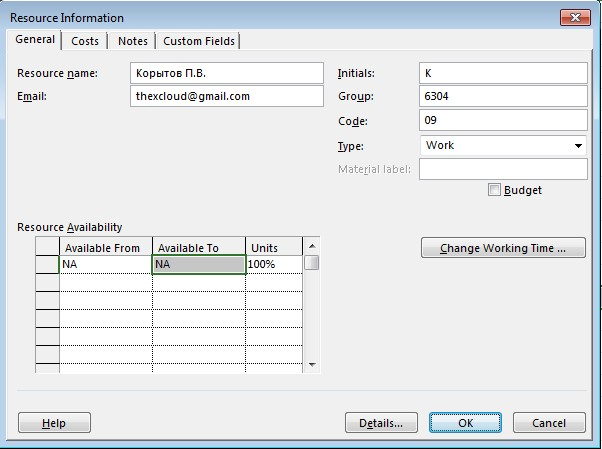
\includegraphics[width=\textwidth]{img/S001.jpg}
        \caption{Создание трудового ресурса}%
        \label{img:res_cr}
    \end{figure}
    
    \item На основе коммитов GitHub и записей Trello относительно лабораторных работ составлен план выполнения. Результат представлен на~\ref{img:plan}
    \begin{figure}[h]
        \centering
        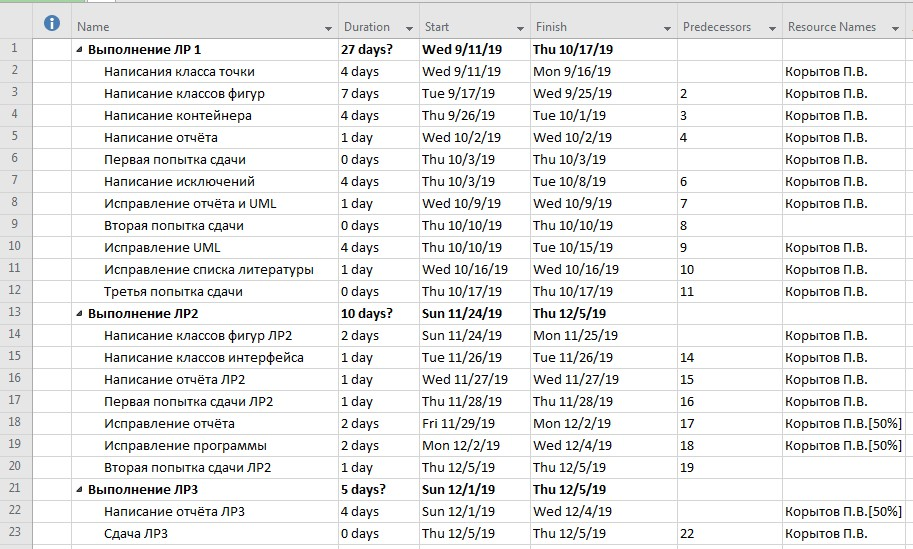
\includegraphics[width=\textwidth]{img/S002.jpg}
        \caption{План выполнения лабораторных работ}%
        \label{img:plan}
    \end{figure}
    \FloatBarrier{}
    
    Попытки сдачи установлены как Milestone.

    \item По созданному плана построена диаграмма Ганта. На диаграмме включено отображение названий задач. Диграмма Ганта для ЛР1 представлена на рис.~\ref{img:gantt1}, для ЛР2--3 --- на рис.~\ref{img:gantt2}

    \begin{figure}[h]
        \centering
        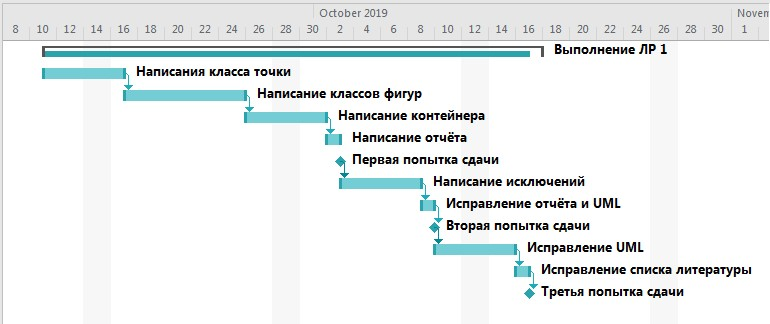
\includegraphics[width=\textwidth]{img/S003.jpg}
        \caption{Диаграмма Ганта для ЛР1}%
        \label{img:gantt1}
    \end{figure}
    
    \begin{figure}[h]
        \centering
        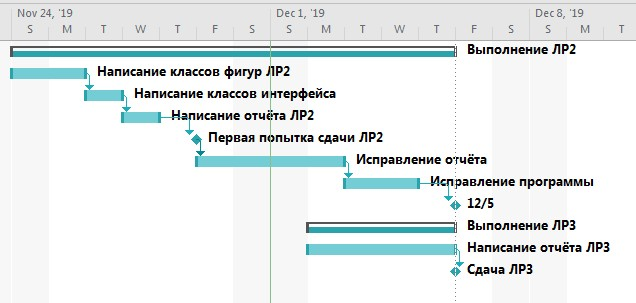
\includegraphics[width=\textwidth]{img/S004.jpg}
        \caption{Диаграмма Ганта для ЛР2--3}%
        \label{img:gantt2}
    \end{figure}
    
    \FloatBarrier{}
    
    \item Построен сетевой график. В свернутом виде график представлен на рис.~\ref{img:network}.

    \begin{figure}[h]
        \centering
        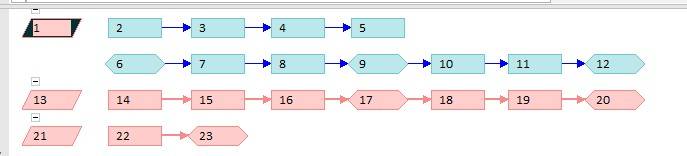
\includegraphics[width=\textwidth]{img/S005.jpg}
        \caption{Сетевой график в свернутом виде}%
        \label{img:network}
    \end{figure}
    
    График экспортирован в формат PDF;\@ полная версия представлена в приложении А.
\end{enumerate}
\subsection{Характеристики}
\subsubsection{Типы задач}
\begin{itemize}
    \item Task (обычная)
    \item Recurring (повторяющаяся)
    \item Summary
    \item Milestone
\end{itemize}

\subsubsection{Параметры задач}
\begin{itemize}
    \item Название
    \item Процент завершения
    \item Начало, конец, длительность
    \item Параметры отображения
    \item Ручной/автоматический режим планирования
    \item Предшественники.\\
    Для каждого:
    \begin{itemize}
        \item ID
        \item Название
        \item Тип:
        \begin{itemize}
            \item Finish-To-Start
            \item Start-To-Finish
            \item Finish-To-Finish
            \item Start-To-Start
        \end{itemize}
        \item Задержка
    \end{itemize}
    \item Ресурсы.\\
    Для каждого:
    \begin{itemize}
        \item Имя
        \item Количество
    \end{itemize}
    \item Deadline
    \item Пометить как milestone
    \item Заметки
    \item Произвольные поля
\end{itemize}

\subsubsection{Параметры ресурсов}
\begin{itemize}
    \item Имя
    \item E-mail, инициалы, группа, код
    \item Тип:
    \begin{itemize}
        \item Work
        \item Material
        \item Cost
    \end{itemize}
    \item График работы
    \item Стоимость
    \begin{itemize}
        \item Standart Rate
        \item Overtime Rate
        \item Effective Rate
        \item Per Use Cost
    \end{itemize}
    \item Заметки
    \item Произвольные поля
\end{itemize}

\subsection{Анализ}
\begin{enumerate}
    \item Включено отображение стоимости работ. Результаты на рис.~\ref{img:cost}
    \begin{figure}[h]
        \centering
        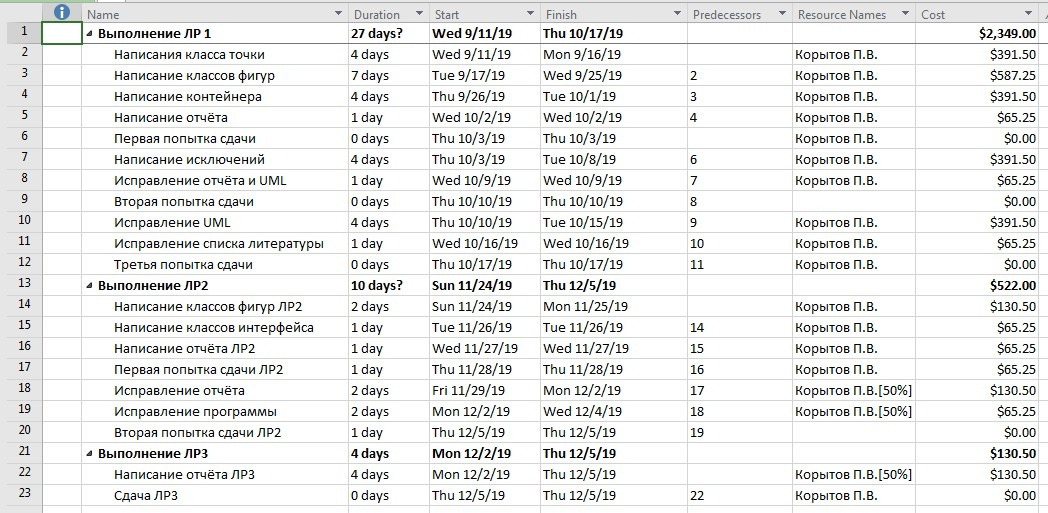
\includegraphics[width=\textwidth]{img/S006.jpg}
        \caption{Стоимость задач}%
        \label{img:cost}
    \end{figure}
    \FloatBarrier{}
    \item Создан ряд встроенные отчётов. Некоторые отчёты представлены на рисунках далее.
    \begin{figure}[h]
        \centering
        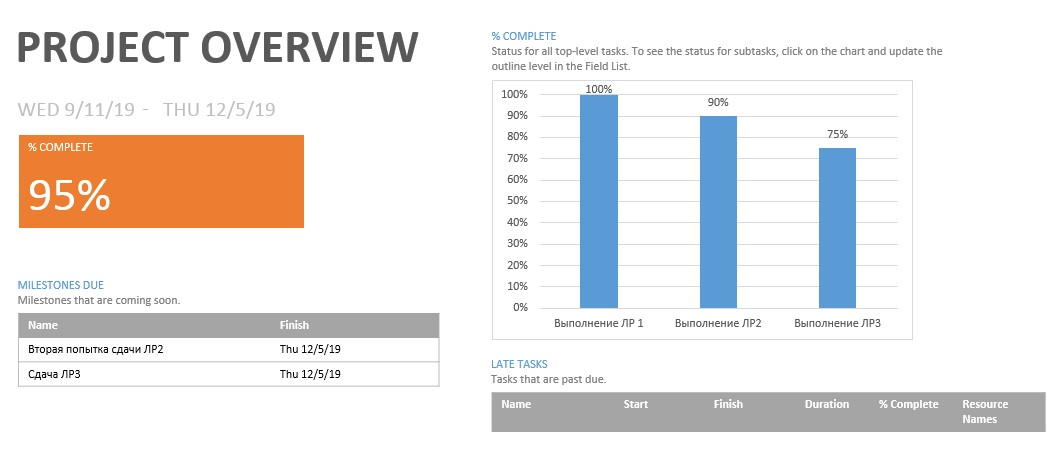
\includegraphics[width=\textwidth]{img/S007.jpg}
        \caption{Отчёт по проекту}%
        \label{img:report:project}
    \end{figure}
    
    \begin{figure}[h]
        \centering
        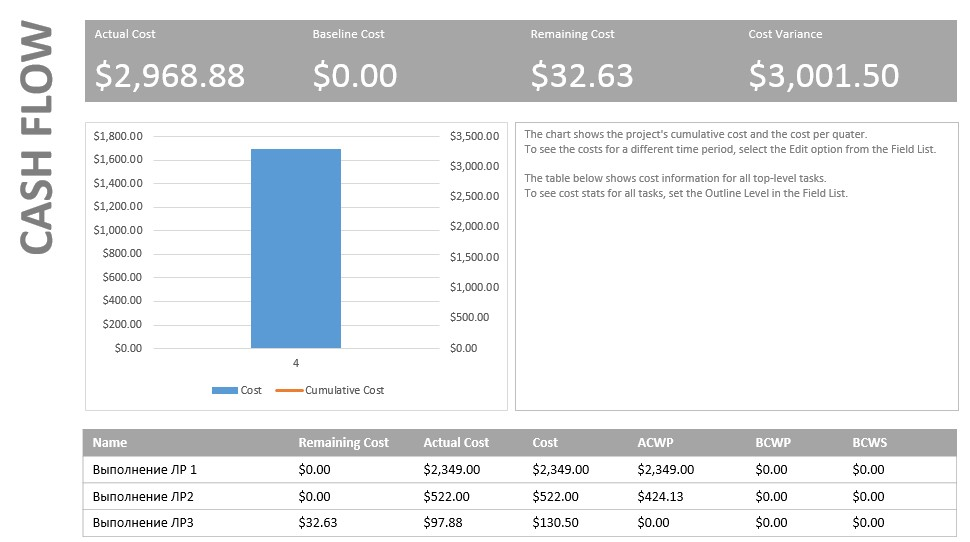
\includegraphics[width=\textwidth]{img/S008.jpg}
        \caption{Отчёт по затратам}%
        \label{img:report:cost}
    \end{figure}
    
    \begin{figure}[h]
        \centering
        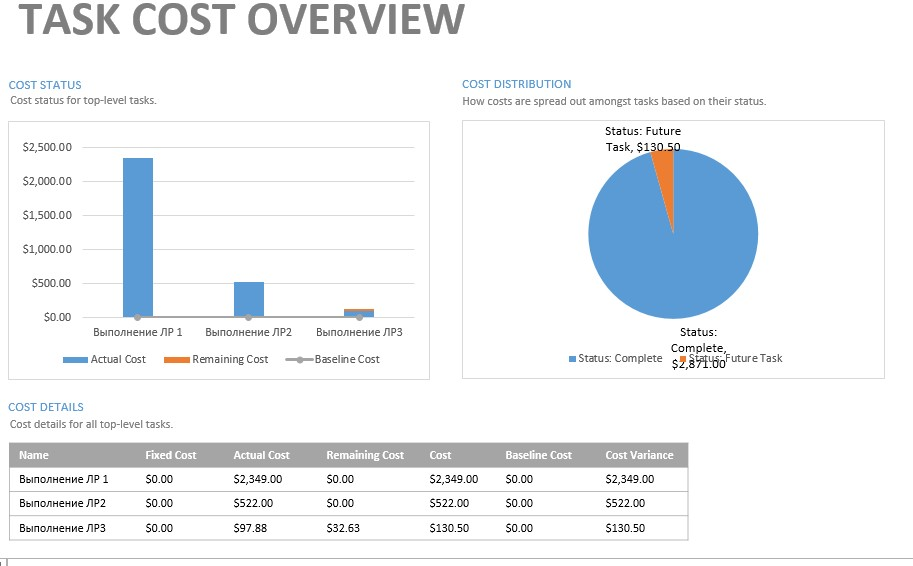
\includegraphics[width=\textwidth]{img/S009.jpg}
        \caption{Затраты на задачи}%
        \label{img:report:task_cost}
    \end{figure}

\end{enumerate}

\section{Вывод}
Произведено изучение способов планирования с помощью Microsoft Project 2019. Изучено использование диаграм Ганта и сетевых графиков.

\StartAddons{}

\newpage
\phantomsection{}
\addcontentsline{toc}{section}{Приложение А. Сетевой график}
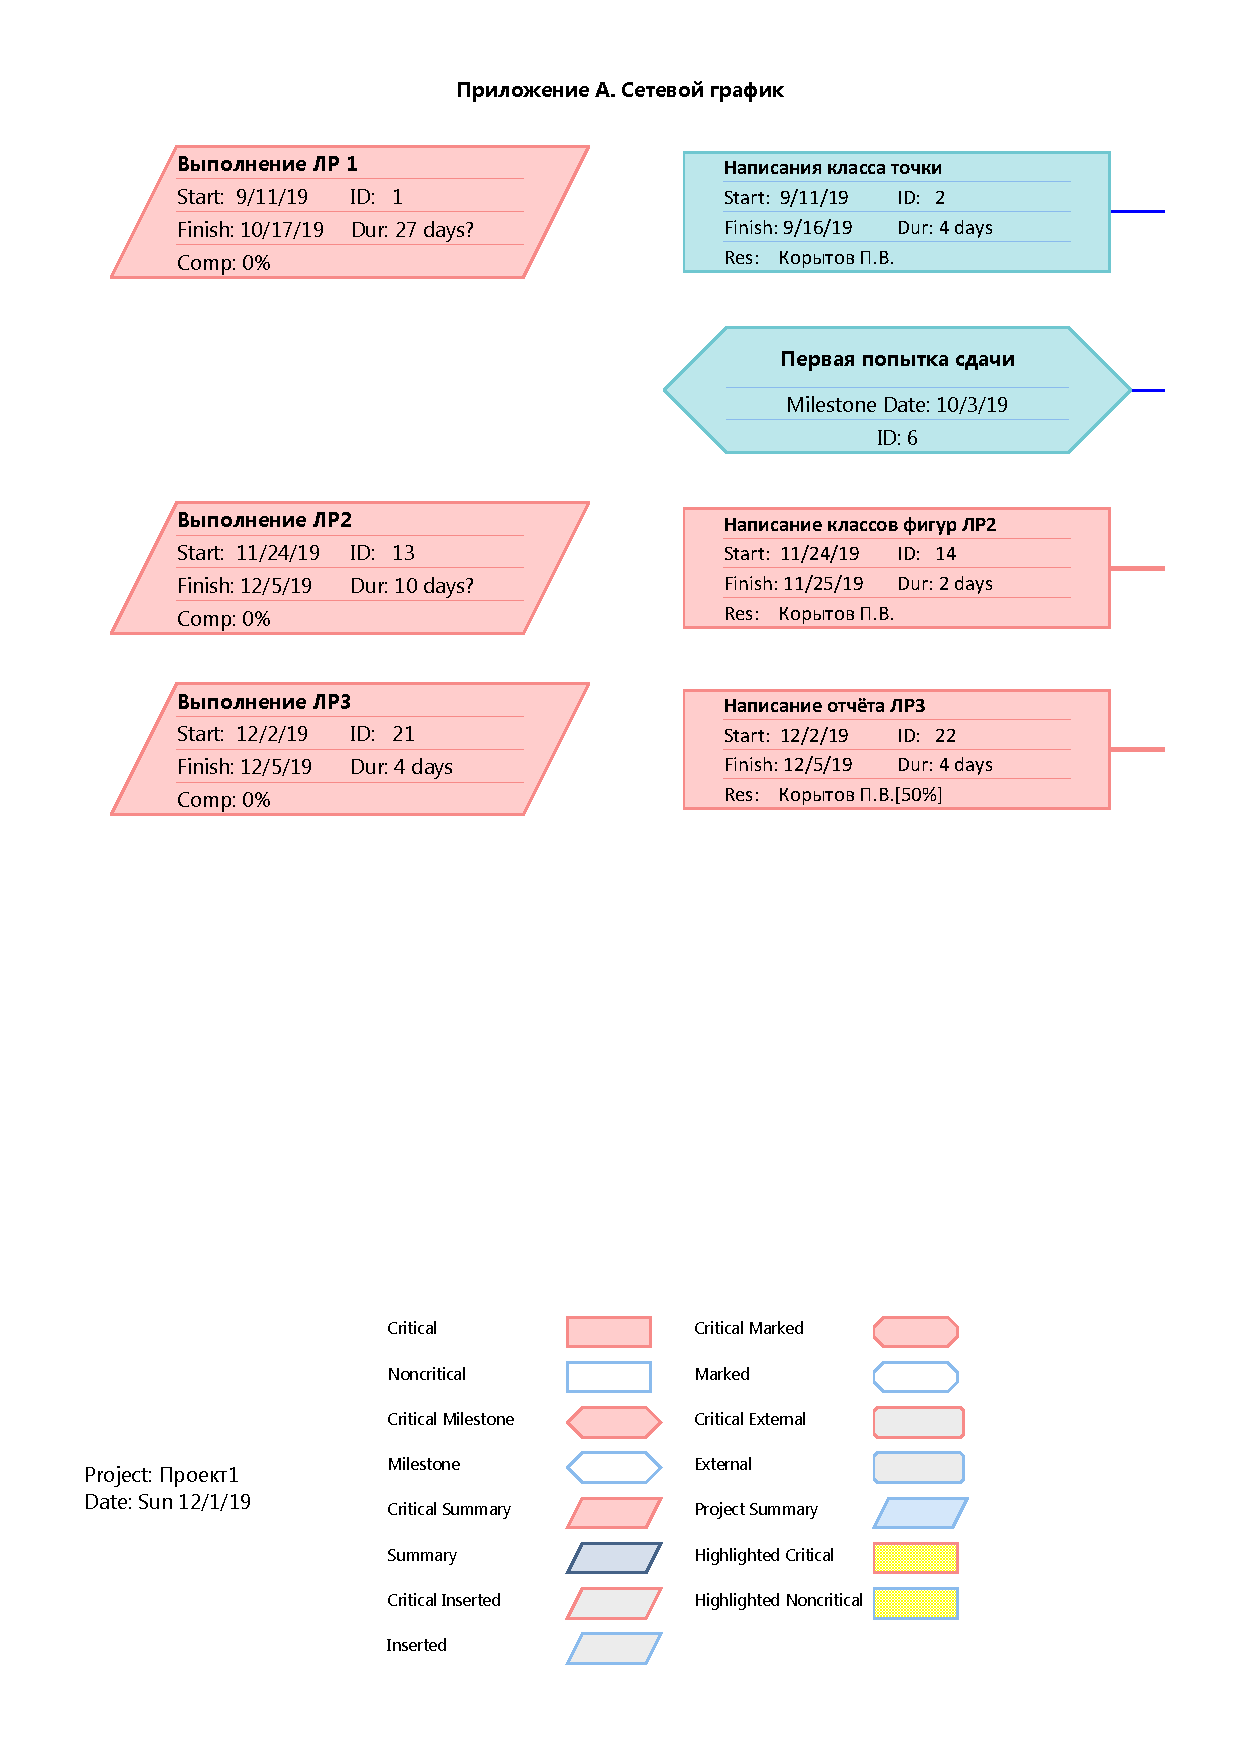
\includepdf[pages=-]{./pdf/Network.pdf}
\end{document}
